\documentclass[12pt,a4paper]{article} 
\usepackage{graphicx}
\begin{document}

\section{Flask}
\subsection{Definisi Flask}
Flask merupakan micro web framework yang ditulis dalam bahasa pemrograman Python. Flask disebut micro framework karena tidak membutuhkan tools tertentu. Framework ini juga tidak mempunyai database abstraction layer, validasi form, atau komponen lainnya yang dimana sudah menyediakan library pihak ketiga yang menyediakan fungsi lain. Akan tetapi, framework flask mendukung extension yang dapat menambah fitur aplikasi seakan-akan mereka diimplementasikan dalam flask itu sendiri.
\subsection{Instlasi Flask}
\subsubsection{On Linux}
Untuk melakukan instalasi flask, ada beberapa tahap yang harus dilakukan yaitu :
\begin{enumerate}
\item Pastikan anda sudah menginstal pyhton baik pyhton versi 2.x maupun 3.x. Jika belum instal, instal terlebih dahulu.

\item Untuk melakukan instalasi flask, kita harus membuat sebuah virtual environment lalu instal flask di dalamnya. Berikut adalah cara instal virtual enviroment / virtualenv.

\$ sudo apt-get install python-virtualenv

\item Lalu, buat satu direktori di hard disk kita untuk tempat pengerjaan project. 

\$ mkdir myproject

\$ cd myproject

\item Setelah itu, kita masuk ke direktori yang sudah di buat sebelumnya dan jalankan terminal untuk menjalankan virtualenv untuk membuat virtualenv di dalam direktori tersebut. Berikut adalah cara menjalankan virtualenv.

\$ virtualenv venv

New python executable in venv/bin/python

Installing setuptools, pip............done.

\item Lalu, berikut adalah cara untuk mengaktifkan virtualenv.

\$ . venv/bin/activate 

dan jika ingin menonaktifkannya, berikut caranya 

\$ deactivate

\item Selanjutnya, kita melakukan penginstalan flask

\$ pip install Flask
\end{enumerate}
\subsubsection{On Mac OS}
1. Instal pip terlebih dahulu menggunakan perintah :

	python get-pip.py

2. Selanjutnya instal flask dengan menggunakan perintah berikut :

	sudo pip install Flask

3. Sekarang, jalankan Simple.py untuk memastikannya berfungsi dengan menggunakan perintah berikut :

	python simple.py

Lalu, jalankan di web browser dengan perintah :

http://127.0.0.1:5000/

ketika sudah selesai, hentikan server dengan menekan kontrol-C.
\subsubsection{On Windows}

1.	Pertama, bukalah command prompt lalu ketikan perintah: pip install virtualenv

2.	Lalu, buatlah folder untuk aplikasi dengan cara mengetikan perintah: mkdir myproject.
Myproject bisa diganti dengan nama lain sesuai keinginan.

3.	Setelah itu, ketikan perintah untuk masuk ke dalam folder myproject: cd myproject. Lalu ketikan perintah: virtualenv flask

4.	Kemudian, ketikan perintah untuk masuk ke dalam folder myproject: cd myproject. Dan ketikan perintah: virtualenv flask

5.	Kemudian, ketikan perintah untuk menginstal flask sebagai berikut:
\begin{figure}[ht]
\centerline{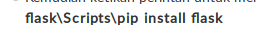
\includegraphics[scale=1]{../figures/3instal.png} }

\caption{Instalasi Flask} 
\label{Flask}
\end{figure}

Pada gambar \ref{Flask} dijelaskan bahwa perintah instal flask

6.	Lalu, buat direktori app di folder myproject dengan perintah: mkdir app

7.	Kemudian masuk ke folder app dan buat folder baru bernama: static, templates dengan perintah mkdir. Sehingga dalam folder app terdapat folder static dan template.

8.	Dan instalasi selesai.

\subsection{Perbedaan Flask}
\hspace{1cm} Flask adalah salah satu microframework yang dapat digunakan di pyhton yang di buat dengan toolkit wsgi dan jinja2. Tentunya flask itu sendiri memiliki banyak perkembangan dari versi pertama saat ia di publikasikan hingga yang terbaru. Disini saya akan menjelaskan tentang sedikit perbedaan antara flask versi 1,0 dan flask versi 0.12. Berikut adalah perbedaannya :
Berikut adalah tabel \ref{table:perbedaan} perbedaan flask.
\begin{table}[h]
\caption{Perbedaan Flask}

\centering
\begin{tabular}{ccc}
\hline
&Flask 1.0&Flask 0.12\\
\hline
Python version&tidak mendukung python versi 2.6 dan 3.3&Support Python 2.6 dan 3.3\\
\hline
Release Date&26 April 2018&21 Desember 2016\\
\hline
\end{tabular}
\label{table:perbedaan}
\end{table}

\end{document}
